\section{Renforcement des modèles}
\label{sec:amelioration_modele}
Dans ce paragraphe, nous présentons des améliorations mises en place
pour les modèles indexés par le temps et les modèles à événements du
\RCPSP~et du \CECSP. 

Dans un premier temps, nous nous sommes intéressé aux modèles à temps
discret pour lesquels nous proposons des inégalités valides déduites
directement du raisonnement énergétique présenté aux
paragraphes~\ref{sec:cumu_propag} et~\ref{sec:ER_CECSP}. En effet, ces modèles restent les modèles 
les plus efficaces pour résoudre le \CECSP~ou le \RCPSP, ceci étant
principalement dû à la qualité relative de leur relaxation. 

Cependant, les limitations de ces modèles nous ont poussé à nous
intéresser plus particulièrement à l'amélioration des modèles à
événements. En effet, le nombre de variables et de contraintes de ces
modèles dépend de la taille de l'horizon de temps du problème. Ce
nombre peut donc s'avérer très important si l'horizon de temps est grand.
De plus, dans les modèles indexés par le temps du \CECSP~, la
discrétisation de l'horizon de temps conduit à une réduction de
l'espace des solutions et peut donc mener à des solutions
sous-optimales (voir exemple~\ref{exemple_NE},
page~\pageref{exemple_NE}). 

Pour améliorer les relaxations linéaires des modèles à événements, nous
avons étudié le polyèdre défini par l'ensemble de toutes les
affectations possibles des variables binaires pour une seule activité,
pour lequel nous exhibons un ensemble minimal d'inégalités permettant
de le décrire. De plus, plusieurs ensembles d'inégalités valides sont
proposées pour contribuer à l'amélioration des performances des
modèles à événements.
 
\subsection{Amélioration des modèles indexés par le temps}
\label{sec:ER_TI}
Dans ce paragraphe, nous montrons comment est utilisé le
raisonnement énergétique décrit au paragraphe~\ref{sec:ER_CECSP} pour
exhiber des inégalités valides pour les modèles de programmation
linéaire mixte indexés par le temps du \RCPSP~et du \CECSP. Nous
commençons par détailler le cas du \CECSP~avant de montrer comment
appliquer le même raisonnement pour le \RCPSP.

Pour intégrer le raisonnement énergétique dans les modèles indexés par
le temps, nous utilisons l'équation qui se trouve au centre de ce
raisonnement (cf. équation~\eqref{eq:centerRE}). Soit $\I$ l'ensemble des
intervalles d'intérêt du raisonnement énergétique, alors l'équation
s'écrit:  
\begin{align} 
  SL(t_1,t_2) &\ge 0 \quad \forall [t_1,t_2] \in \I \nonumber\\
  \Rightarrow \bb + \sum_{\substack{j\in \A\\j\neq i}}\bb[j] &\le
  R(t_2-t_1)\quad \forall [t_1,t_2] \in \I \nonumber
\end{align}  

Soit $CR: \mathbb{R} \times \H \times \H \rightarrow \mathbb{R}$ qui
associe à une quantité d'énergie $w$ et à un intervalle $[t_1,t_2]$,
la quantité de ressource minimale à consommer dans $[t_1,t_2]$ pour
apporter à une activité une énergie $w$ (voir
équation~\eqref{eq:conv_CECSP}). En considérant toutes les
expressions possibles pour $\bb$ et en utilisant les variables
$x_{it}$ et $y_{it}$ pour activer ou non l'équation correspondant à la
consommation minimale de ressource dans $[t_1,t_2]$, nous obtenons les
inégalités suivantes: 
\begin{align}
  &\left(1-\sum_{t\le t_1}x_{it} - \sum_{t\ge t_2}y_{it}\right) \, \conv[W_i] +
    \sum_{j\neq i} \bb[j] \le R(t_2-t_1) \nonumber\\
  & \hspace{9.55cm} \forall i \in \A,\ \forall [t_1,t_2] \in \I
    \label{total}
\end{align}

L'inégalité~\eqref{total} représente le cas où l'intervalle
$[\ES,\LE]$ est complètement inclus dans $[t_1,t_2]$. En effet,
les différents cas possibles sont: 
\begin{itemize}
\item l'activité commence après $t_1$ et finit avant $t_2$. Dans ce
  cas-là, l'inégalité devient: 

$\conv[W_i] +\sum_{j\neq i} \bb[j] \le
  R(t_2-t_1)$. Ceci correspond au cas où la contrainte est activée. 
\item l'activité commence avant $t_1$ et finit avant $t_2$. Ici,
  l'inégalité devient: $\sum_{j\neq i} \bb[j] \le R(t_2-t_1)$ et ceci
  est vérifié quel que soit $i$ et $[t_1,t_2]$. Ce cas correspond au
  cas où la contrainte n'est pas activée. 
\item l'activité commence après $t_1$ et finit après $t_2$. Ce cas est
  similaire au précédent. 
\item l'activité commence avant $t_1$ et finit après
  $t_2$. L'inégalité s'écrit alors: $\sum_{j\neq i} \bb[j]-\conv[W_i]
  \le R(t_2-t_1)$. Ce cas est aussi similaire au second. 
\end{itemize}

\begin{align}
&\left(x_{i,\ES} + y_{i,\LE} -1 \right) \, \conv[W_i-f_i(\bmax)\left(t_1-\ES + \LE
-t_2\right)] \nonumber \\
&+ \sum_{j\neq i} \bb[j] \le R\left(t_2-t_1\right) \hspace{4.35cm} \forall i \in
{\cal A},\ \forall [t_1,t_2] \in \I  \label{both}
\end{align}

L'inégalité~\eqref{both} correspond au cas où l'activité est centrée,
i.e. $\ES\le t_1<t_2 \le \LE$ et $W_i-\left(t_1-\ES + \LE -t_2\right)
\ge f_i(\bmin)(t_2-t_1)$. Dans ce cas, l'inégalité sera activée si et
seulement si l'activité commence à $\ES$ ($x_{i,\ES}=1$) et finit à
$\LE$ ($y_{i,\LE}=1$). 

\begin{align}
&\left(x_{i,\ES} + \sum_{t=t_1}^{t_2}y_{it} -1\right) \,
\conv[W_i-f_i\left(\bmax\right)\left(t_1-\ES\right)]+ \nonumber\\
&\sum_{j\neq i} \bb[j] \le R\left(t_2-t_1\right) \hspace{4.75cm} \forall i \in
  {\cal A},\ \forall [t_1,t_2] \in \I
\label{left}
\end{align}

L'inégalité~\eqref{left} correspond au cas où l'activité est calée à
gauche, i.e. exécutée à $\bmax$ pendant l'intervalle
$[\ES,t_1]$. Cette inégalité est activée quand l'activité commence à
$\ES$ et finit dans l'intervalle $[t_1,t_2]$. 

\begin{align}
&\left(\sum_{t=t_1}^{t_2}x_{it} + y_{i,\LE}-1\right) \,
\conv[W_i-f_i\left(\bmax\right)\left(t_2-\LE\right)]\nonumber\\
& + \sum_{j\neq i} \bb[j] \le R\left(t_2-t_1\right) \hspace{4.29cm} \forall i \in
{\cal A},\ \forall [t_1,t_2] \in \I
\label{right}
\end{align} 

L'inégalité~\eqref{right} correspond au cas où l'activité est calée à
droite, i.e. exécutée à $\bmax$ pendant l'intervalle
$[t_2,\LE]$. Cette inégalité est activée quand l'activité commence
dans l'intervalle $[t_1,t_2]$ et finit a $\LE$.

\begin{align}
&\left(\sum_{t\le t_1}x_{it} + \sum_{t\ge t_2}y_{it} -1 \right) \,
  \bmin\left(t_2-t_1\right) + \sum_{j\neq i} \bb[j] \nonumber\\
& \le R\left(t_2-t_1\right)\hspace{7cm} \forall i \in {\cal A},\ \forall [t_1,t_2]
\in \I
\label{min}
\end{align}

Enfin, l'inégalité~\eqref{min} correspond au cas où l'activité est
exécutée à $\bmin$ durant l'intervalle $[t_1,t_2]$. Cette inégalité
assure que si l'activité commence à $t_1$ ou avant et finit à $t_2$ ou
après alors la quantité de ressource disponible dans $[t_1,t_2]$ est
suffisante pour exécuter l'activité à $\bmin$ durant tout cet
intervalle.


Notons que ces inégalités peuvent aussi être définies dans le cas du
\RCPSP. Dans ce cas là, nous devons appliquer le même raisonnement
pour chaque ressource. Cependant, il y aura seulement trois cas à
considérer: l'activité est calée à gauche, l'activité est calée à
droite et l'activité est en cours d'exécution durant l'intervalle
$[t_1,t_2]$. Ceci donne les inégalités suivantes:
\begin{multline} \left(x_{i,\ES} + \sum_{t=t_1}^{t_2}y_{it} -1\right)
\, r_{ik}p_i^+(t_1)+ \sum_{j\neq i} \bb[j] \le R\left(t_2-t_1\right)
\qquad \\ \forall i \in {\cal A},\ \forall k \in \R ,\ \forall
[t_1,t_2] \in \I
    \label{RCPSP_left}
\end{multline} \vspace{-1.3cm}
\begin{multline} \left(\sum_{t=t_1}^{t_2}x_{it} + y_{i,\LE}-1\right)
\, b_ip_i^-(t_2) + \sum_{j\neq i} \bb[j] \le R\left(t_2-t_1\right)
\qquad \\ \forall i \in {\cal A},\ \forall k \in \R ,\ \forall
[t_1,t_2] \in \I
    \label{RCPSP_right}
\end{multline} \vspace{-1.3cm}
\begin{multline} \left(\sum_{t\le t_1}x_{it} + \sum_{t\ge t_2}y_{it}
-1 \right) \, b_i\left(t_2-t_1\right) + \sum_{j\neq i} \bb[j] \le
R\left(t_2-t_1\right) \qquad \\ \forall i \in {\cal A},\ \forall k \in
\R ,\ \forall [t_1,t_2] \in \I
    \label{RCPSP_min}
\end{multline}
avec $p_i^+(t_1)$ et $p_i^-(t_2)$ comme définis dans le
paragraphe~\ref{sec:cumu_propag} pour le \CUSP. 

De telles inégalités ont été proposées dans le cadre du modèle
préemptif sur les ensembles admissibles~\cite{BD}. Ces inégalités sont
ajoutées au modèle indexé par le temps du \CECSP~et du \RCPSP~et les
performances de ces modèles avec ou sans ces inégalités sont évaluées
dans le chapitre~\ref{sec:expe} afin de montrer leur intérêt.
 
Les modèles à temps discret sont particulièrement efficaces pour le
\RCPSP~et le \CECSP. Cependant, ces modèles possèdent des limitations
qui sont décrites dans la section suivante. 



\subsection{Amélioration des modèles à événements}
\label{sec:amelioration_OO}
Dans ce paragraphe, nous présentons les améliorations possibles des
modèles à événements. Dans un premier temps, nous montrons que le
modèle start/end possède de meilleures relaxations que le modèle
on/off, puis nous présentons un ensemble d'inégalités que nous pouvons
rajouter au modèle on/off pour renforcer sa relaxation. Cet ensemble
d'inégalités est ensuite utilisé pour donner une description minimale
du polyèdre défini par l'ensemble de toutes les affectations possibles
des variables binaires $z_{ie}$ pour une seule activité. 

D'autres ensembles d'inégalités, permettant l'ajout de nouvelles
contraintes au modèle, sont ensuite présentées , la suppression des
coefficients big-$M$ dans les contraintes existantes ou l'amélioration
des contraintes existantes. Dans ce paragraphe, nous présentons les
résultats pour le \CECSP~car, dans la plupart des cas, le remplacement
de $\Em=\{1,\dots,2n-1\}$ par $\{1,\dots,n\}$ suffit à l'adaptation de
la preuve au \RCPSP. Cependant, lorsque ce n'est pas le cas ou que le
résultat n'a pas été prouvé pour le \RCPSP, nous le précisons.

\subsubsection{Comparaison des relaxations linéaires}

Pour montrer que le modèle start/end possède de meilleures relaxations
linéaires que le modèle on/off, nous commençons par montrer que le
modèle start/end possède des relaxations au moins aussi bonnes que
celles du modèle on/off. Pour cela, il suffit de  montrer que toute solution du 
modèle start/end, entière ou non, est solution du modèle on/off. Ceci
peut être fait en écrivant les variables $z_{ie}$ en fonction des
variables $x_{ie}$ et $y_{ie}$ et nous avons la relation suivante,
décrite dans le paragraphe~\ref{sssection:OO_CECSP}: 
\begin{equation}
\label{SEversOO}
z_{ie} = \sum_{f=1}^e x_{if} -  \sum_{f=1}^e y_{if} \quad \forall i
\in \A,\ \forall e\in \Em
\end{equation}

Il nous reste maintenant à montrer que les relaxations du modèle
on/off ne sont pas aussi bonnes que celles du modèle start/end. Pour
cela, nous relâchons les contraintes d'intégrité des deux modèles et
nous trouvons une solution pour la relaxation du modèle on/off qui
n'en est pas une pour la relaxation du modèle start/end. 

Considérons le sous-modèle formé des
équations~\eqref{start_CECSP_OO}, \eqref{preem1_CECSP_OO} et
\eqref{preem2_CECSP_OO} et le sous-modèle formé des
équations~\eqref{start_CECSP_SE}, \eqref{end_CECSP_SE},
\eqref{SEversOO} et de l'ensemble d'équations suivant: $\sum_{f=1}^e
y_{if} +\sum_{f=e}^n x_{if}\le 1,\ \forall i \in \A$. Clairement, si
nous trouvons une solution pour le premier sous-modèle qui n'en est
pas une pour le second, ceci montrera bien que les relaxations du modèle
on/off ne sont pas aussi bonnes que celles des modèles start/end. En
effet, toute solution d'un des sous-modèles est solution du modèle
entier (start/end ou on/off) en considérant l'instance suivante:
$\forall i \in \A,\ \ES=0,\ \LE=T,\ \bmin=0,\ \bmax=1,\ W_i=1,\
f_i(b_i(t))=b_i(t)$ et $B=n$. 

Nous nous plaçons dans le cas où le nombre d'activités est de 2. Alors,
nous avons $|\E|=4$.  Dans la suite, les tâches sont notées par les
indices $a$ et $b$ et les événements par $0,\ 1,\ 2$ et $3$.

Nous constatons tout d'abord que $z_a=(0,6\,;\,0\,;\,0,7\,;\,0)$ est bien une
solution du sous-modèle on/off. 

Nous devons maintenant montrer que le sous modèle start/end ne possède
pas de solution avec $z_a=(0,6\,;\,0\,;\,0,7\,;\,0)$. Pour cela, étudions les contraintes du
modèle qui n'impliquent que l'activité $a$:

\begin{align} &x_{a0}+x_{a1}+x_{a2}+x_{a3}= 1 \label{c9}\\
              &y_{a0}+y_{a1}+y_{a2}+y_{a3}= 1 \label{c10}\\
              &y_{a0}+x_{a0}+x_{a1}+x_{a2}+x_{a3}\le1 \label{c11}\\
              &y_{a0}+y_{a1}+x_{a1}+x_{a2}+x_{a3}\le1 \label{c12}\\
              &y_{a0}+y_{a1}+y_{a2}+x_{a2}+x_{a3}\le1 \label{c13}\\
              &y_{a0}+y_{a1}+y_{a2}+y_{a3}+x_{a3}\le1 \label{c14}\\
              &0.6=x_{a0}-y_{a0}\label{c17}\\
              &0=x_{a0}-y_{a0}+x_{a1}-y_{a1}\label{c18}\\
              &0.7=x_{a0}-y_{a0}+x_{a1}-y_{a1}+x_{a2}-y_{a2}\label{c19}\\
              &0=x_{a0}-y_{a0}+x_{a1}-y_{a1}+x_{a2}-y_{a2}+x_{a3}-y_{a3}\label{c20}
\end{align}

Clairement, dans le modèle start/end, nous avons les contraintes
suivantes: $x_{a3}=0$ et $y_{a0}=0$. Donc, les contraintes~(\ref{c17})
et~(\ref{c20}) impliquent que $x_{a0}=0,6$ et $y_{a3}=0,7$. 

Or, la contrainte~(\ref{c18}) implique $y_{a1}=0,6+x_{a1}$
et la contrainte~(\ref{c9}) implique $0,6+x_{a1}+x_{a2}=1 \Rightarrow
x_{a2}=0,4-x_{a1}$. 

La contrainte~(\ref{c12}) peut donc s'écrire
$0,6+2x_{a1}+x_{a2}\le 1 \Rightarrow 1+x_{a1}\le 1 \Rightarrow
x_{a1}=0$. 

Ceci implique $x_{a2}=0,4$ et $y_{a1}=0,6$, et l'on obtient
une contradiction avec la contrainte~(\ref{c10}) puisque $0+0,6+y_{a2}+0,7>1$.

Donc, nous avons bien montré que le modèle start/end possède en
théorie de meilleures relaxations que le modèle on/off. Cependant, si
nous ajoutons un ensemble particulier d'inégalités à ce modèle, ceci
n'est plus le cas. Ces inégalités sont décrites dans le paragraphe
suivant.


\subsubsection{Inégalités de non préemption}
\label{sec:nonPreem}
Dans ce paragraphe, nous présentons un ensemble d'inégalités que nous
utilisons pour donner une description minimale du polyèdre défini par
l'ensemble de toutes les affectations possibles des variables binaires
$z_{ie}$ pour une seule activité. 

L'ensemble d'inégalités, appelées inégalités de non préemption, est
défini comme suit. Puisque, dans tout ordonnancement réalisable,
chaque activité doit être exécutée sans préemption, $z_{ie}$ doit
satisfaire:
\begin{equation}
  \sum_{e_u \in {\cal F}} (-1)^{u} z_{i,e_u} \le 1
\label{non_preem_ineg}
\end{equation}
où ${\cal F}=\{e_0,e_1,\dots,e_{2v}\}$ est un sous-ensemble ordonné de
cardinalité impaire de $\E^*=\Em$.  

Soit le polyèdre $ZP_i=\{z_i \in [0,1]^{\E^*}\ | \ z_i\text{ satisfait
\eqref{start_CECSP_OO} et \eqref{non_preem_ineg}}\}$ et soit
$ZQ_i=\mathrm{conv}\{z_i \in \{0,1\}^{\E^*}\ | \ z_i\text{ satisfait
\eqref{start_CECSP_OO},\eqref{preem1_CECSP_OO} et
\eqref{preem2_CECSP_OO}}\}$. Nous allons montrer le théorème suivant: 

\begin{theo}
$ZP_i=ZQ_i$.
\end{theo}

\begin{proof}

Dans un premier temps, nous rappelons le lemme de Farkas que nous
utiliserons plus tard dans la preuve. 

\begin{lemma}[Lemme de Farkas]
\label{Farkas_Lemma}
Soit $A$ une matrice de taille $m \times n$ et $b$ un vecteur de
$\mathbb{R}^m$. Il existe un vecteur $x \in \mathbb{R}^n$ vérifiant
$Ax = b$ si et seulement si pour tout vecteur $y \in \mathbb{R}^m$
tel que $ y^TA\le 0$ on a $y^Tb \le 0$. 
\end{lemma}

Nous allons exhiber un ensemble d'inégalités linéaires décrivant
$ZQ_i$. Pour cela, commençons par remarquer que les sommets de $ZQ_i$
sont exactement les vecteurs de dimension $|\E^*|$ suivants:
\[
z_{i,e}^{uv}=\left\{
\begin{array}{ll}
1 & \text{ si }u \le e \le v\\
0 & \text{ sinon}
\end{array}
\right. \qquad \forall u,\ v \in \E^*,\ u \le v
\]
Donc, un point $\overline{z}_i \in ZQ_i$ si et seulement si le système
linéaire suivant admet une solution réalisable:
\begin{align}
& \sum_{u\le v} z_{i,e}^{uv} \lambda_{uv} = \overline{z}_{i,e} & &
\forall e \in \E^* \label{kis1}\\
&\sum_{u \le v} \lambda_{uv} =1 & & \label{kis2}\\
&\lambda \ge 0 & & \label{kis3}
\end{align}

Or, d'après le lemme de Farkas, le
système~\eqref{kis1}--\eqref{kis3} admet une solution réalisable si et
seulement si $\forall \mu \in \mathbb{R}^{|\E^*|}$ tel que: 
\begin{equation}
\sum_{e=u}^{v} \mu_e + \mu_0 \le 0, \quad u \le v 
\label{kis4} 
\end{equation}
$\mu$ satisfait aussi la condition suivante: 
\begin{equation}
\sum_{e \in \E^*} \mu_e \overline{z}_{i,e}+ \mu_0 \le 0
\label{kis5}
\end{equation}
Donc, puisque les rayons extrêmes du cône caractérisé par~\eqref{kis4}
définissent toutes les inégalités linéaires requises pour décrire
$ZQ_i$, il suffit, pour prouver le théorème, de trouver tous ces
rayons extrêmes. 

Nous allons ensuite montrer qu'il existe une bijection entre les
rayons extrêmes du cône~\eqref{kis4} vérifiant~\eqref{kis5} et les
inégalités de $ZP_i$.

Pour trouver les rayons extrêmes du cône~\eqref{kis4}, il suffit de
considérer les trois cas suivants: 
\paragraph{\boldmath $\mu_0 > 0$.} Quitte à normaliser, nous pouvons
suppposer que $\mu_0=1$. Dans ce cas-là, pour tout $e \in \E^*$, nous
avons $\mu_e \le -1$. En effet, ceci est déduit de~\eqref{kis4} en
considérant l'équation pour $u=v=e$. Alors, en prenant
$\mu_e=-1,\forall e \in \E^*$, ~\eqref{kis5} implique:
\[ \sum_{e \in \E^*} - \overline{z}_{i,e} \le -1 \] D'après le lemme
de Farkas, ceci est une inégalité valide pour $ZQ_i$. On peut
remarquer que ces inégalités sont équivalentes
à~\eqref{start_CECSP_OO}. 
\paragraph{\boldmath $\mu_0 = 0$.} Alors, nous avons toujours un cône
dont les rayons extrêmes sont les vecteurs unité négatifs de
$\mathbb{R}^{\E^*}$. Ces rayons extrêmes nous donnent les inégalités
$z_{i,e} \ge 0$ qui sont les contraintes de non négativité valides
pour $ZQ_i$.
\paragraph{\boldmath $\mu_0 < 0$.} Quitte à normaliser, nous pouvons
supposer que $\mu_0=-1$. Nous allons prouver que dans ce cas, il
existe une bijection entre les points extrêmes du polyèdre $H$ défini
par:
  \begin{equation} \sum_{e=u}^{v} \mu_e \le 1 \quad u \le
    v \label{kis6}
  \end{equation} 
et les inégalités~\eqref{non_preem_ineg}. Comme~\eqref{kis6}
implique~\eqref{kis5}, ceci montrera bien la bijection entre les
rayons extrêmes de~\eqref{kis4} vérifiant~\eqref{kis5} et les
inégalités~\eqref{non_preem_ineg}.

  Dans un premier temps, nous montrons que le vecteur formé des
  coefficients de la partie gauche de chaque inégalité
  de~\eqref{non_preem_ineg} est une solution de~\eqref{kis6}
  correspondant à un point extrême de $H$. 

  Soit ${\cal F}=\{e_0,e_1,\dots,e_{2v}\}$ un ensemble d'événements
  vérifiant $e_i<e_{i+1}$ pour $i=0,\dots,2v-1$. Le vecteur
  $\overline{\mu}$ formé des coefficients de la partie gauche de chaque
  inégalité de~\eqref{non_preem_ineg} est défini par:
  \[ \overline{\mu}_e=\left\{ 
      \begin{array}{ll}
        (-1)^u & \text{ si } e=e_u \in \cal F \\
        0 & \text{ si } e \in \E^* \setminus \cal F
      \end{array}
    \right.
  \]
  Pour prouver que $\overline{\mu}$ est une solution de~\eqref{kis6}
  correspondant à un point extrême de $H$, nous exhibons un
  sous-système $L$ de~\eqref{kis6} 
  contenant $|\E^*|$ inégalités linéairement indépendantes telles que
  chaque inégalité de $L$ soit vérifiée à l'égalité par
  $\overline{\mu}$. 

  Le sous-système $L$ est formé des inégalités suivantes: 
  \begin{align*}
    & \sum_{e=u}^{e_0} \mu_e \le 1 & & u=1,\dots, e_0-1\\
    & \sum_{e=e_{2v}}^u \mu_e \le 1& & u=e_{2v},\dots,|\E^*|
  \end{align*}
  De plus, $L$ contient l'ensemble d'inégalités suivant, défini pour
  tout ensemble formé de 3 événements consécutifs
  $e_{2u},e_{2u+1},e_{2u+2} \in \cal F$:   
  \begin{align*}
    & \sum_{e=e_{2u}}^{e_{2u+2}} \mu_e \le 1 & & \\
    & \sum_{e=e_{2u}}^t \mu_e \le 1& & t=e_{2u},\dots,e_{2u+2}-1\\
    & \sum_{e=t}^{e_{2u+2}} \mu_e \le 1& & t=e_{2u+1}+1,\dots,e_{2u+2}-1
  \end{align*} 
  On peut facilement vérifier que le système ci-dessus est formé de
  $|\E^*|$ inégalités linéairement indépendantes et que
  $\overline{\mu}$ vérifie chacune d'entre elle à l'égalité et ceci
  prouve notre affirmation. 

  Nous montrons maintenant que toute solution $\overline{\mu}$
  correspondant à un point extrême de $H$ équivaut à une inégalité
  de~\eqref{non_preem_ineg}. Dans un premier temps, remarquons que la
  matrice formée par les coefficients de la partie gauche
  de~\eqref{kis6} est totalement unimodulaire. En effet, les colonnes
  de cette matrice peuvent être réordonnées de telle sorte que chaque
  ligne ne contienne que des $1$ consécutifs. Donc, tout sommet de
  ce polyèdre est un vecteur à valeurs entières. Nous remarquons aussi
  que $\overline{\mu}_e\le 1,\ \forall e \in \E$, puisque $\mu_e \le 1$
  est une inégalité de~\eqref{kis6} ($u=v$) pour tout $e \in \E^*$.
  
  Soit $u_1$ le premier indice tel que $\overline{\mu}_{u_1} \neq 0$. Nous
  affirmons que $\overline{\mu}_{u_1}=1$. Supposons que ce ne soit pas
  le cas, i.e. $\overline{\mu}_{u_1} \le -1$ (les coordonnées de
  $\overline{\mu}$ sont entières). Puisque $\overline{\mu}$ est un point
  extrême de $H$, il existe un sous-ensemble $L$ formé de $|\E^*|$
  inégalités linéairement indépendantes de~\eqref{kis6} qui sont
  satisfaites à l'égalité par $\overline{\mu}$. 

  Remarquons que $L$ doit contenir une inégalité impliquant la
  variable $\mu_{u_1}$. En effet, si ce n'est pas le cas, cette variable
  peut être arbitrairement fixée à une valeur négative et toujours
  satisfaire toutes les inégalités de $L$. Et donc $\overline{\mu}$ ne
  serait pas un point extrême de $H$ ce qui est une contradiction. Comme
  $\overline{\mu}_e=0$ pour $e< u_1$, une telle inégalité doit être de
  la forme $ \sum_{e=u_1}^{v_1} \mu _e \le 1$. Comme elle doit être
  satisfaite par $\overline{\mu}$ à l'égalité et que $\overline{\mu}_e
  \le 1$, nous avons que $\overline{\mu}$ doit contenir au moins deux
  coordonnées $q_1$ et $q_2$ tels que $ u_1 \le q_1 \le q_2 \le v_1$
  avec $\overline{\mu}_{q_1}=\overline{\mu}_{q_2}=1$ et
  $\overline{\mu}_{e}=0$ pour $q_1 < e < q_2$. Mais, dans ce cas-là,
  $\overline{\mu}$ violerait l'inégalité $\sum_{e=q_1}^{q_2} \mu_e \le
  1$ et ceci est une contradiction. Donc, la première coordonnée non
  nulle de $\overline{\mu}$ doit 
  prendre la valeur $1$. 
  
  La seconde coordonnée non nulle, disons
  $u_2$, ne peut prendre la valeur $1$ par le même raisonnement que
  précédemment. Donc, cette valeur doit être négative et
  entière. Mais, dans ce cas-là, nous pouvons suivre la même
  argumentation que précédemment pour montrer que $u_2$ doit
  apparaître dans une des inégalités de $\ell \in L$ et aboutir à la même
  contradiction que précédemment. Donc, la seconde coordonnée non nulle
  de $\overline{\mu}$ doit être égale à $-1$. De plus, $\ell$ doit
  contenir une inégalité impliquant une variable $\mu_{u_3}$ de valeur
  $1$ dans $\overline{\mu}$. En effet, dans le cas contraire,
  $\overline{\mu}$ ne peut satisfaire $\ell$ à l'égalité. Si nous
  poursuivons cette argumentation tant que $\mu$ possède des
  coefficients non nuls après $u_3$, nous reconnaissons la suite de
coefficients $1/-1$ présente dans~\eqref{non_preem_ineg}.
\end{proof}

Nous avons donc défini un ensemble d'inégalités permettant une
description complète du polyèdre formé par les vecteurs $z_i$ solution
du modèle on/off. Cependant, nous ne pouvons ajouter directement ces
inégalités au modèle car leur nombre est exponentiel. Dans le
chapitre~\ref{sec:expe}, nous présenterons un algorithme de 
séparation polynomial qui nous permettra de définir un algorithme de
branch-and-cut pour le \CECSP~et le \RCPSP~(rappelons que les
résultats ci-dessus sont valides dans le cas du \RCPSP~en posant
$\E^*=\{1,\dots,n\}$). 

Le paragraphe suivant présente d'autres inégalités valides pour le
\CECSP~et le \RCPSP. 

\subsubsection{Autres inégalités valides}

\label{sec:maxDist}
Dans ce paragraphe, nous décrivons plusieurs ensembles d'inégalités
valides pour le \RCPSP~ et le \CECSP. Dans la suite, nous considérons
qu'un événement correspond à une et une seule date de début/fin,
i.e. $\forall e \in \Em[1]$, il existe une et une seule activité $i$
vérifiant $(z_{i,e-1}-z_{ie}=1) \vee (z_{ie}-z_{i,e-1}=1)$. Cela est
toujours possible puisque $|\E|=2n$. De plus, l'ajout de cette
supposition ne change pas la véracité de ce qui précède. 

\paragraph{Séparation maximale entre deux événements} 
Les inégalités définies dans ce paragraphe sont des inégalités bornant
supérieurement la valeur de $t_{e+1}- t_e, \forall e\in \Em$. Pour
définir ces inégalités, nous étudions les fenêtres de temps de chaque
date de début et de fin d'une activité, i.e. $[\ES,\LS]$ et
$[\EE,\LE],\ \forall i \in \A$. L'idée principale repose sur le fait
que, dans chacun de ces intervalles, un événement doit forcément avoir
lieu. De ce fait, nous savons qu'il y a au moins deux événements
consécutifs dans l'union de deux fenêtres de temps consécutives. 

Soit ${\cal D}$ l'ensemble de toutes les fenêtres de temps, i.e. ${\cal
D}=\{[\ES,\LS] , [\EE,\LE],\ \forall i \in \A\}$. Nous commençons par
trier les intervalles de $\cal D$ suivant la règle suivante: 
$[a,b] \le [c,d]
\Leftrightarrow a<c \lor \left( a=c \land b\le d\right)$

Alors, soit $\underline{{\cal D}_e}$ (resp. $\overline{{\cal D}_e}$)
la borne inférieure (resp. supérieure) de l'intervalle ${\cal D}_e$,
nous avons la propriété suivante:
\begin{equation} \label{sep_CECSP_OO} 
t_{e+1}-t_e \le \max(\overline{{\cal D}_e},\overline{{\cal D}_{e+1}}) -
\min(\underline{{\cal D}_e},\underline{{\cal D}_{e+1}}) \qquad \forall e \in {\cal E}\setminus\{2n\}
\end{equation}

\begin{ex}
\label{ex:evt_sep} Considérons l'ensemble d'intervalles suivant:
\begin{center}
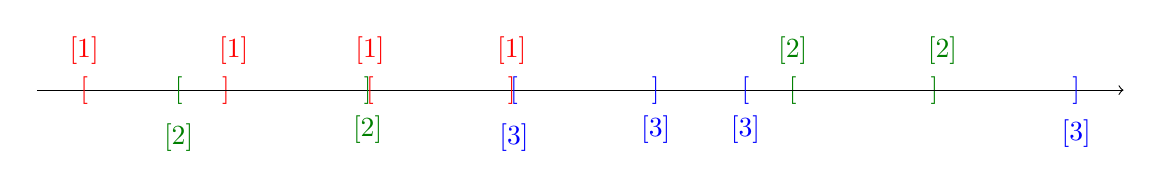
\begin{tikzpicture} [yscale=0.8,xscale=0.6] \node (O) at (0,0) {};

\draw[->] (0,0) -- (23,0);
 \draw (1,0) node[red] {$[$} node[above=0.2cm,red]
{$\ES[1]$}-- +(0:3cm)node[red] {$]$} node[right=0.1cm,above=0.2cm,red]{$\LS[1]$};

\draw(7.05,0) node[red] {$[$} node[above=0.2cm,red] {$\EE[1]$}-- +(0:3cm) node[red]
{$]$} node[above=0.2cm,red] {$\LE[1]$};
 \draw (3,0) node[Green] {$[$} node[below=0.3cm,Green]
{$\ES[2]$}-- +(0:4cm) node[Green] {$]$} node[below=0.2cm,Green] {$\LS[2]$};
 \draw
(16,0) node[Green] {$[$} node[above=0.2cm,Green] {$\EE[2]$}-- +(0:3cm) node[Green] {$]$}
node[right=0.1cm,above=0.2cm,Green] {$\LE[2]$};
 \draw(10.1,0) node[blue] {$[$}
node[below=0.3cm,blue] {$\ES[3]$}-- +(0:3cm) node[blue] {$]$} node[below=0.2cm,blue]
{$\LS[3]$};
 \draw (15,0) node[blue] {$[$} node[below=0.2cm,blue] {$\EE[3]$}--
+(0:7cm) node[blue] {$]$} node[below=0.25cm,blue] {$\LE[3]$};

\end{tikzpicture}
\end{center}

Après avoir trié les intervalles, nous obtenons:
$[\ES[1],\LS[1]] \le [\ES[2],\LS[2]] \le
[\EE[1],\LE[1]] \le [\ES[3],\LS[3]] \le 
[\EE[3],\LE[3]] \le [\EE[2],\LE[2]] $.

Alors, nous avons l'ensemble de contraintes suivantes:

\begin{itemize}
\item $t_2-t_1 \le \LS[2]-\ES[1]$
\item $t_3-t_2 \le \LE[1]-\ES[2]$
\item $t_4-t_3 \le \LS[3]-\EE[1]$
\item $t_5-t_4 \le \LE[3]-\ES[3]$
\item $t_6-t_5 \le \LE[3]-\EE[3]$
\end{itemize}

\end{ex}

Notons aussi que l'ensemble d'inégalités
$\underline{{\cal D}_e} \le t_e \le \overline{{\cal D}_e}$ peut ne pas
être valide. En effet, ici $t_6$ peut correspondre à la fin de
l'activité $3$ et $t_5$ à la fin de l'activité $2$, alors que
${\cal D}_5=[\EE[3],\LE[3]] \le [\EE[2],\LE[2]]={\cal D}_6$. On aurait
alors $\underline{{\cal D}_6} \le t_5 \le \overline{{\cal D}_6}$.

Ces contraintes peuvent être ajoutées au modèle on/off ou utilisées
comme borne supérieure sur la valeur de $\bmin(t_{e+}-t_e)$
dans~\eqref{bmin_CECSP_OO}. L'inégalité se réécrit donc comme:
\[ b_{ie} \ge \bmin(t_{e+}-t_e) - \bmin\left(\max(\overline{{\cal
D}_e},\overline{{\cal D}_{e+1}}) - \min(\underline{{\cal
D}_e},\underline{{\cal D}_{e+1}})\right)(1-z_{ie})\qquad \forall (i,e)
\in {\cal A}\times{\cal E}
\]

Ces inégalités peuvent être généralisées à tout sous-ensemble de $k$
intervalles ordonnés $\{{\cal D}_{e_1},\dots,{\cal D}_{e_k}\}$ avec
$t_{e_k}-t_{e_1} \le \max(\overline{{\cal D}_{e_1}},\overline{{\cal
D}_{e_k}}) - \min(\underline{{\cal D}_{e_k}},\underline{{\cal
D}_{e_1}}) $.

\paragraph{Date maximale d'un événement}


Une idée similaire à celle décrite dans le paragraphe précédent peut
être utilisée pour ordonner les événements et calculer des bornes
supérieures sur leur date. 

Pour faire cela, nous commençons par trier les bornes supérieures des
fenêtres de temps de chaque activité, i.e. $\LS$ et $\ES,\ \forall i
\in \A$, par ordre croissant. Alors, puisqu'un événement doit avoir
lieu dans chaque fenêtre de temps, i.e. avant chaque borne supérieure de
chaque fenêtre, nous pouvons déduire une borne supérieure sur la date
de chaque événement.

En effet, soit ${\cal UP}$ l'ensemble formé de toutes les bornes
supérieures de toutes les fenêtres de temps. Alors, nous avons la
propriété suivante: 
\begin{equation} \label {Bte_CECSP_OO} t_e \le {\cal UP}_e \qquad
\forall e \in {\cal E}
\end{equation}

\begin{ex} 
Considérons les intervalles définis dans
l'exemple~\ref{ex:evt_sep}. Alors, nous pouvons déduire l'ensemble de
contraintes suivantes:

\begin{itemize}
\item $t_1 \le \LS[1]$
\item $t_2 \le \LS[2]$
\item $t_3 \le \LE[1]$
\item $t_4 \le \LS[3]$
\item $t_5 \le \LE[2]$
\item $t_6 \le \LE[3]$
\end{itemize}
\end{ex}

Comme précédemment, nous pouvons utiliser ces inégalités comme
contraintes additionnelles des modèles à événements ou les utiliser
à la place de  $T$ dans les contraintes \eqref{twx_CECSP_OO}
et\eqref{twy2_CECSP_OO}. Les contraintes s'écrivent alors: 
\begin{align*}
& \ES z_{ie}\le t_e \le \LS(z_{ie}-z_{i,e-1})+(1-(z_{ie}-z_{i,e-1})){\cal UP}_e 
 & & \forall e \in \E\setminus \{1\},\ \forall i \in {\cal
   A}\\
&t_e \le \LE(z_{i,e-1}-z_{ie})+(1-(z_{i,e-1}-z_{ie})){\cal UP}_e  & & \forall e
 \in \E\setminus \{1\},\ \forall i \in {\cal
   A}
\end{align*}

Pour le \RCPSP, $t_n$ correspond à borne supérieure sur la durée
totale du projet, i.e. sur $T$.

\paragraph{Inégalités valides dérivées du problème de sac-à-dos}

Le rendement minimal de chaque activité pouvant être positif, nous
pouvons considérer les contraintes de type sac-à-dos suivantes pour
tout $e \in \Em$ et les transformer facilement en inégalités valides: 
\begin{equation}
\sum_{i\in \A^+} \bmin z_{ie} \leq B  \qquad  \forall e \in \E
\end{equation}
où $\A^+$ est le sous-ensemble d'activités avec $\bmin > 0$. 


\paragraph{Inégalités de cliques}

Les inégalités de clique permettent de modéliser le fait que plusieurs
variables binaires $z_{ie}$ ne peuvent prendre la valeur $1$
simultanément. Ces inégalités, déjà établies dans le cas du
\RCPSP~\cite{CAVT_clique}, correspondent aux sous-ensembles
disjonctifs d'activités. Elles sont facilement adaptables au cas du
\CECSP~et sont définies de la manière suivante. Soit $C$ un ensemble
minimal d'activités ne pouvant s'exécuter en parallèle, i.e. telles que
$\sum_{i \in C} \bmin > B$, alors l'ensemble d'inégalités suivantes
est valide pour le \CECSP: 
\begin{equation} 
\sum_{i\in C} z_{ie}  \le |C| -1 \qquad \forall C,\ \forall e \in \E
\end{equation}


Différentes techniques permettant l'intégration des inégalités
ci-dessus seront présentées et comparées dans le
chapitre~\ref{sec:expe}.